%\chapter{提案手法}
\chapter{シンボルテーブルを用いた検知手法の提案}

\section{検知手法へのアプローチ}
検知手法を定めるために,IoTデバイス上で普段の動作とマルウェアがダウンロードされ実行されたあとの動作の違いを明らかにする.その後,Miraiを実際に動作をさせデバイス上で行われている動作の解析を行う.実行コマンド,プロセスの2つのログデータの収集を行い,マルウェアが実行される前と後の相違点を明らかにする.

\section{Miraiソースコードを用いた稼働調査}
Miraiの挙動の稼働調査としてWeb上で公開されているMiraiのソースコード\cite{code}を用いてマルウェアが感染する際の感染動作とC\&Cサーバーとの通信が行われ,攻撃命令を待機するまでのマルウェアの動作を確認した.MiraiがIoTデバイスに感染する様子を確認するために用いた,VMを用いた解析環境を図\ref{fig:kaiseki}に示す.Miraiをダウンロードさせ実行させるための感染端末,Loader,C\&Cサーバー,MySQLの4つを用意した.MySQLにC\&Cサーバーの管理ユーザを登録しC\&Cサーバーと感染端末の通信状態を確認できるようにした.Loaderが感染端末にTelnetログインを行い,感染端末の通信が確立される.ログイン後に実行されるコマンドの収集を行い、表\ref{tab:malware}に示すコマンド列を得た.
\begin{table}[t]
   \caption{マルウェアによる実行コマンド}
   \label{tab:malware}
   \centering
\begin{tabular}{p{7cm}}
\hline
/bin/busybox wget;\\
/bin/busybox wget http://192.168.32.10:80/bins/mirai.x86 -O -\textgreater dvrHelper;\\
/bin/busybox chmod 777 dvrHelper;\\
./dvrHelper telnet.x86;\\
\hline
\end{tabular}
\end{table}
表\ref{tab:malware}のようにMiraiはバイナリファイルをダウンロードした際に,バイナリファイルの名称をdvrHelperに変更している.しかし,バイナリファイルの実行後に,psコマンドでプロセス名を確認すると,無作為なプロセス名で動作し,他の端末からTelnetログインが不可になっていることが確認された.Miraiには,DDoS攻撃を行う機能だけではなく,特定のポートを閉じる機能やプロセス名を無作為にする機能が存在することが確認された.
 \begin{figure}[h]
 \centering
    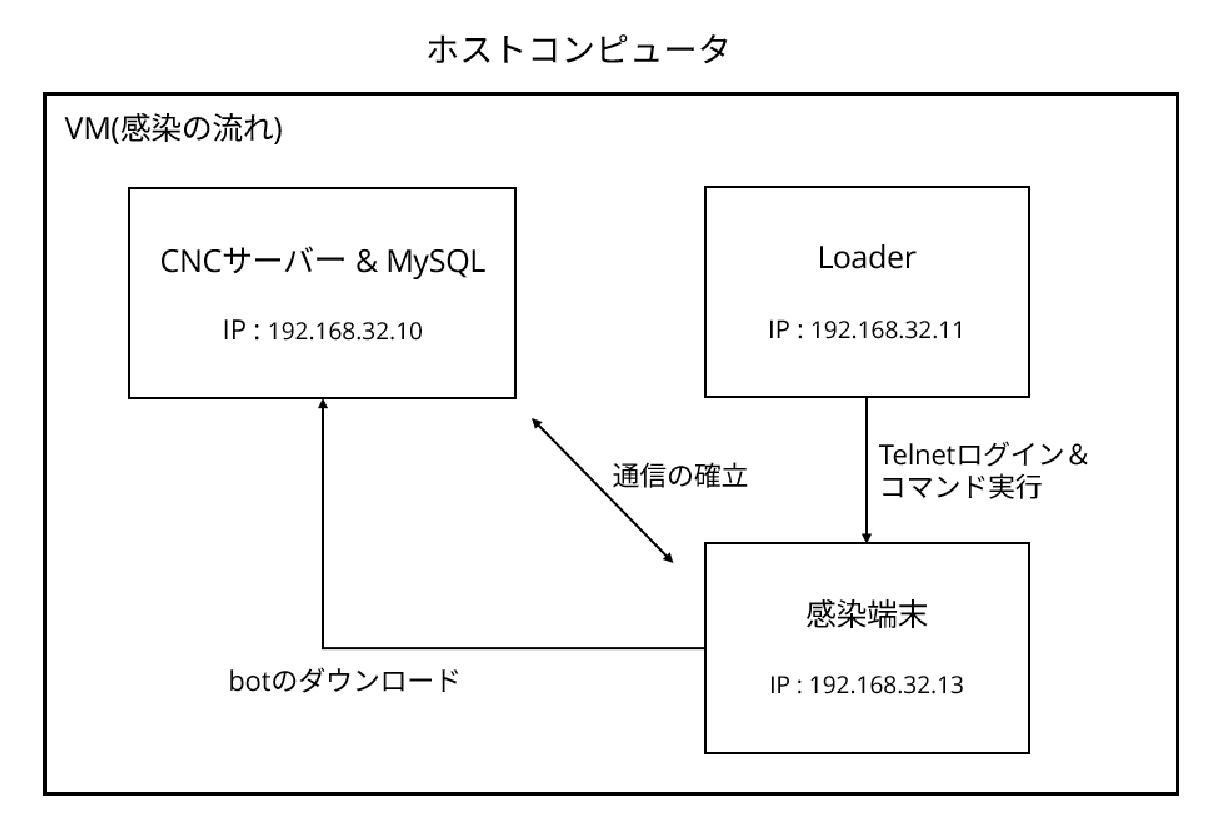
\includegraphics[width=100mm]{figures/VM.eps}
    \caption{Miraiの解析環境}
 \label{fig:kaiseki}
 \end{figure}
 \newpage

\section{シンボルテーブルを用いた検知手法の提案}
計算資源が潤沢でないIoTデバイス上でも実現可能な,Mirai亜種の動作を検知する軽量な表層解析に基づく検知システムを提案する.検知システムの概要を図\ref{fig:symbol}に示す.Miraiとその亜種であるOwariを含めて調査したところ,DDoS攻撃を行うマルウェアについて亜種を含めて同様の機能を持つ,同一のコードが再利用されていることが確認された.そこで,マルウェアが持つ特定の関数の具備を検知条件として定め,この条件を満たすプロセスの稼働を検出することによってマルウェア感染の有無を判定する手法を以下に述べる.\\
シンボルテーブルとは,プログラム内で定義されている変数名,関数名に関する情報が保持されたファイルである.シンボルテーブルを取得することによってプログラム内で使用されている関数名を把握が可能であることからマルウェアが持つ特定の関数の具備したプログラムを検出する.
%IoTデバイス上で動作を行うプロセスのホワイトリストを作成する.ホワイトリストとは,端末上で可動が許可されたプロセスリストのことである.ホスト上の動作しているプロセスを監視し,作成されたホワイトリストをもとに記載がないプロセスを発見する.検知対象となるプロセスを動かしているバイナリファイルのシンボルテーブルを取得し,プロセス名を無作為に変更する等のマルウェアが持つ特定の関数の有無を確認する.マルウェアが有している特定の関数の存在が確認できた場合にはマルエウェアと判断する.

\begin{enumerate}
 \item IoTデバイス上で動作を行うプロセスのホワイトリストを作成する.ホワイトリストとは,端末上で可動が許可されたプロセスリストのことである.
 \item プロセスを監視し、作成されたホワイトリストをもとに記載がないプロセスを発見する.
 \item ホワイトリストにないプロセスに関して,プロセスを動かしているバイナリファイルのシンボルテーブルを取得し,プロセス名を無作為に変更するなどのマルウェアの特定の関数が存在しているか確認を行う.
\item マルウェアが持つ特定の関数の存在が確認できた場合には,マルウェアだと判断を行う.
 \item ホワイトリストにないプロセスに関して,シンボルテーブルの探索が終わった場合には2に戻る
\end{enumerate}

ファイルに備わっているシンボルテーブルを取得する際にホワイトリストを用いる事によって,シンボルテーブルを取得するファイルを限定する.それにより,シンボルテーブルを取得する回数を減らすことが可能でありIoTデバイスの計算資源を節約することができる.検知項目のマルウェアが持つ特定の関数として,DDoS攻撃を行う関数や,事前調査で把握した,プロセス名を無作為にする関数や,特定のポートを閉じる関数などが候補に挙げられる.
 
 \begin{figure}[h]
 \centering
    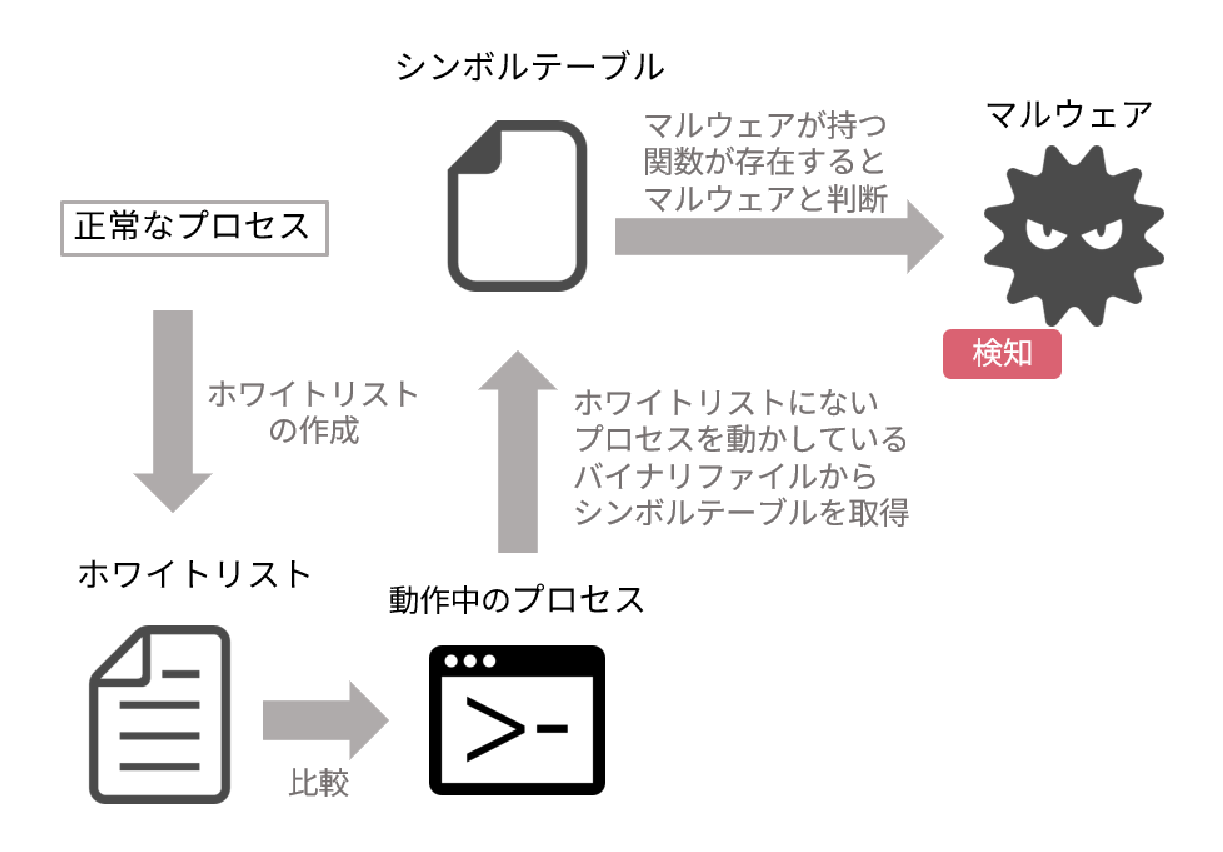
\includegraphics[width=120mm]{figures/system.eps}
    \caption{シンボルテーブルを用いた検知システムの概要}
    \label{fig:symbol}
 \end{figure}
 
\newpage


%掲載したグラフから何を読み取るべきかきちんと数値で言及をする.

\section{マルウェア探索動作による負荷と検知における制約事項}
IoTデバイスは放置されることが多く,常に操作を行っているわけではない.そのため継続的にアンチウィルスソフトウェアなどの検知システムを利用してIoTデバイスにマルウェアがダウンロードされ実行されていないか確認し,IoTデバイスが安全な状態であることを把握する必要がある。検知システムのマルウェア探索動作によって,IoTデバイスの動作が妨げられる可能性がある.IoTデバイス上でMiraiなどDDoS攻撃をおこなうマルウェアが動作している際には,特定のサーバーに対してDDoS攻撃を行ってしまうためIoTデバイスの正常な動作を妨げてまでマルウェアを検知する必要がある.しかし,IoTデバイス上でマルウェアが動作していない状況下において映像,音声,ログなどの様々なデータを伝達するなどのIoTデバイスの本来の動作がマルウェアの探索動作によって阻害されてはならない.そのため,IoTデバイスにマルウェアが動作していない状況下において,提案した検知システムによるマルウェア探索動作がIoTデバイス本来の動作を阻害していないか評価を行う.そして,IoTデバイスでMiraiが動作した場合に,提案した検知システムによって検知が可能であることを評価する.\par
提案手法の稼働に必要なマルウェア探索動作によってIoTデバイス本来の動作が阻害されてないことを評価するために,LinuxOSを対象とする既存のアンチウィルスソフトであるClam AntiVirus(ClamAV)を動作させた状態のCPUとメモリ使用率をそれぞれ基準値とし,提案手法によるマルウェア探索動作の動作負荷について比較を行い,併せて提案手法によってMiraiマルウェアの検知が可能であることを確認した.提案した検知システムによってMiraiが動作していない状況での、CPU,メモリの使用率について調査した.sarと呼ばれるシステムの負荷状況を確認するコマンドを用いて1分間計測を行なった.表\ref{tab:spec}の性能のラズベリーパイを利用し負荷状況を測定した.
\begin{table}[h]
   \caption{評価環境のIoTデバイスのスペック}
   \label{tab:spec}
   \centering
   \begin{tabular}{|l|c|l|l|l|}
   \hline
   \multicolumn{3}{|c|}{Raspberry Pi3} \\ \hline
   OS     & \multicolumn{2}{c|}{Openwrt 4.9.120}                   \\ \hline
   CPU    & \multicolumn{2}{c|}{Quad Core 1.2GHz Broadcom BCM2837} \\ \hline
   MEM    & \multicolumn{2}{c|}{1GB}                               \\ \hline
   \end{tabular}
\end{table}

%!!!!!!!!!!!!!!!!!!!!!!!!!!!!!!!!!!!!!!!!!!!!!!!!!!!!!!!!!!!!!!!!!!!!!!!!!!!!!!!!!!!!!!!
%!評価に用いた評価環境を記載する(まだ記載されていない).対象のIoTデバイスのスペック等々!
%!!!!!!!!!!!!!!!!!!!!!!!!!!!!!!!!!!!!!!!!!!!!!!!!!!!!!!!!!!!!!!!!!!!!!!!!!!!!!!!!!!!!!!!

sarコマンドを用いて得たCPU,メモリの使用率についてClam AntiVirusと提案した検知システムの比較を行った結果が図\ref{fig:symbol_cpu},\ref{fig:symbol_mem}になる.Clam AntiVirusを利用した場合には,平均CPU使用率が25.28\%,メモリ使用率は7.93\%となった.提案した検知手法では,平均CPU使用率が3.03\%,メモリ使用率が7.21\%となった.メモリ使用率は比較対象のClam AntiVirusと提案した検知手法では12.5\%減,CPU使用率は,Clam AntiVirusに対して提案した検知手法は88\%減となったことからマルウェアの可動を検知する目的で一般的によく利用されるClam AntiVirusに比較して提案手法の実装では資源消費が少なく他のプロセスの動作を妨げる可能性は低いと言える.しかし,提案した検知した検知手法は実行形式ファイルに含まれるシンボルテーブルの内容に基づいている為,マルウェアの実行形式ファイルに対してstripコマンドを用いるなどしてシンボルテーブルが削除された場合には検知が行えないという課題がある.

\begin{figure}[h]
 \centering
    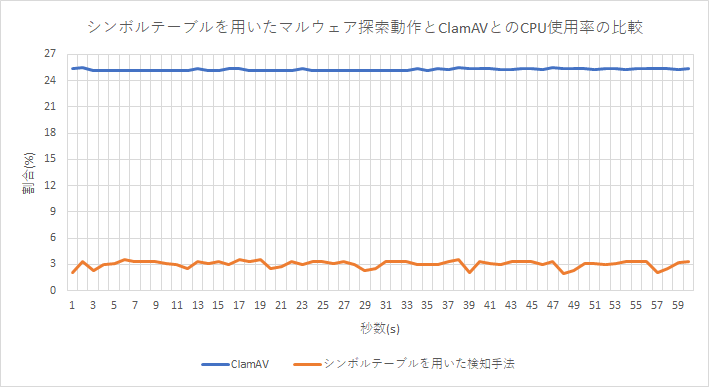
\includegraphics[width=120mm]{figures/cpu.eps}
 \caption{シンボルテーブルを用いたマルウェア探索動作とClamAVとのCPU使用率の比較}
 \label{fig:symbol_cpu}
 \end{figure}
 
 
\begin{figure}[h]
 \centering
    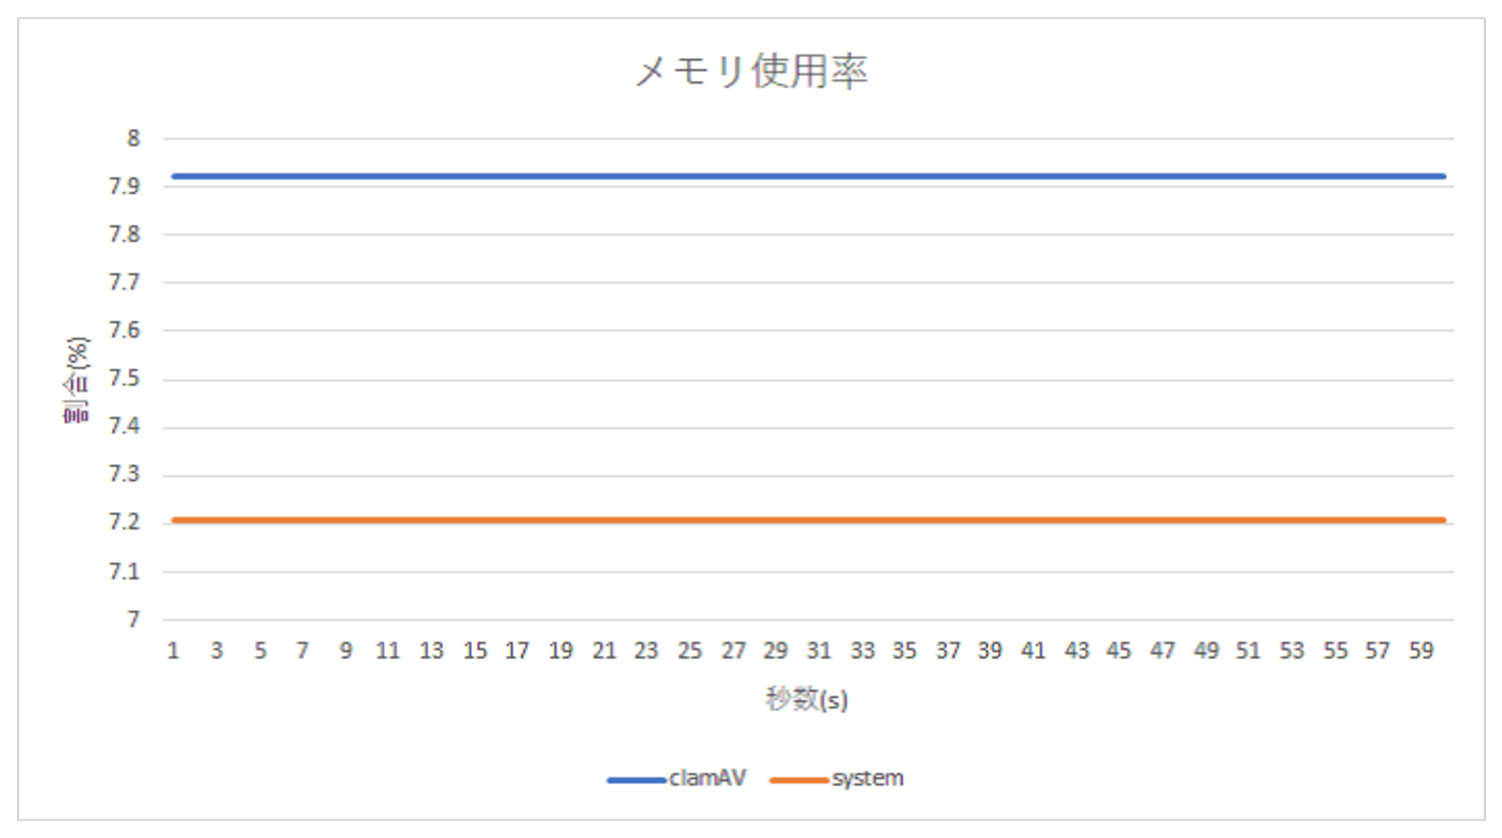
\includegraphics[width=120mm]{figures/mem.eps}
   \caption{シンボルテーブルを用いたマルウェア探索動作とClamAVとのメモリ使用率の比較}
    \label{fig:symbol_mem}
 \end{figure}
